\title{Introductory Electricity, Magnetism, and Optics Practice Problems}
\author{Cyrus Vandrevala}

\documentclass[11pt]{article}
\usepackage{amsmath}
\usepackage[margin=2.5cm]{geometry}
\usepackage[pdftex]{graphicx}

\begin{document}

\maketitle
\tableofcontents
\vspace{50pt}

\subsection*{Useful Constants}
Electron Mass = $9.11 \times 10^{-31}$ kg \\*
Proton Mass = $1.67 \times 10^{-27}$ kg \\*
Elementary Charge = $1.602 \times 10^{-19}$ C \\*
Coulomb's Constant = $8.99 \times 10^9$ Nm$^2$/C$^2$ \\*
Permittivity of Free Space = $8.85 \times 10^{-12} s^4 A^2 / (kg \cdot s^4)$ \\*
Permeability of Free Space = $1.25 \times 10^{-6} m \cdot kg / (s^2 A^2)$ \\*
Speed of Light in a Vacuum = $3 \times 10^8$ m/s \\*
Acceleration Due to Gravity = 9.81 m/s$^2$ \\* \\*
Planck's Constant = $6.626 \times 10^{-34} m^2$kg/s 
1 Astronomical Unit (AU) is the mean distance between the Earth and the Sun $\approx 1.50 \times 10^{11}$ m 

%%%%%%%%%%%%%%%%%%%%%%%%%%%%%%%%%%%%%%%%%%%%%%%%%%%%%%%%%%%%%%%%%%%%%%%%%%%%%%

\pagebreak
\section{Maxwell's Equations}
\vspace{10pt}

\subsection{Displacement Current}
I have a uniform magnetic field and uniform electric field pointing in the $+\hat{z}$-direction.  They are increasing at a constant rate of 10 N/Cs and 30 T/s.  I now draw a circular Amperian surface of radius R in the xy-plane.  What is the displacement current going through the surface? \\* \\*
$\Rightarrow I_D = 10 \mu_o \epsilon_o \pi R^2$

%%%%%%%%%%%%%%%%%%%%%%%%%%%%%%%%%%%%%%%%%%%%%%%%%%%%%%%%%%%%%%%%%%%%%%%%%%%%%%

\pagebreak
\section{Properties of Light}
\vspace{10pt}

\subsection{Michelson-Morley Experiment}
The Michelson-Morley experiment showed that the speed of light in a vacuum is \underline{\hspace{8mm}}. \\* \\*
$\Rightarrow$ Constant

\subsection{Time of Travel \#1}
What is Fermat's principle? \\* \\*
$\Rightarrow$ Fermat's principle states that the path taken by light traveling from one point to another is such that the time of travel is a minimum.  In other words light travels along the path of least time.

\subsection{Time of Travel \#2}
A beam of light travels through 10 m of plastic with an index of refraction of n = 1.50; a second beam of light travels through 13 m of vacuum.  Which beam of light will complete its journey in a shorter amount of time? \\* \\*
$\Rightarrow$ The one travelling through vacuum.

\subsection{Radiation Pressure}
A laser beam of power 5.60 W and diameter 1.30 mm is directed upward at one circular face of a perfectly reflecting cylinder, which is made to "hover" by the beam's radiation pressure.  Each face of the cylinder has an area A = 100 mm$^2$.  The cylinder has a density of 1200 kg/m$^3$.  What is the height (H) of the cylinder?  You may assume that the cylinder is completely contained within the laser beam.

\begin{center}
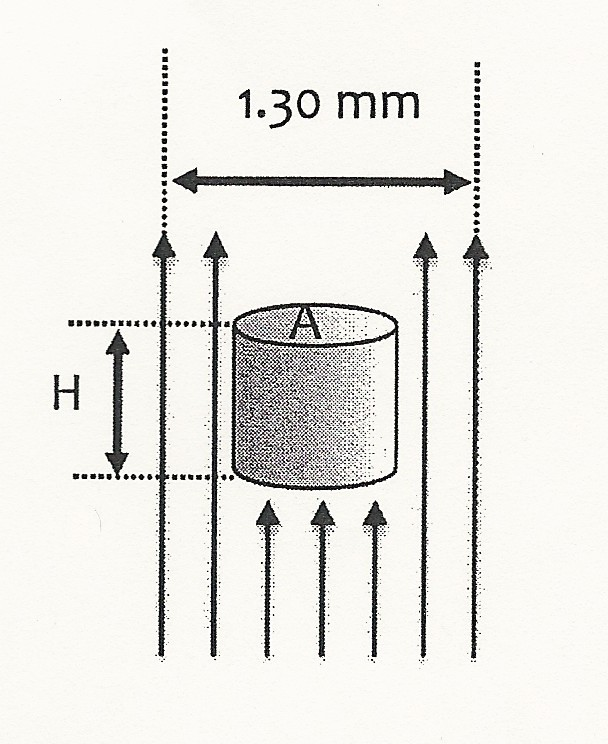
\includegraphics[scale=0.2]{Images/radiation_pressure.jpg}
\end{center}

$\Rightarrow$ H = 1.2 $\mu$m

\subsection{Intensity of Light}
The intensity of sunlight on the Earth is about 1400 W/m$^2$.  What is the intensity of sunlight on Saturn?  Note that earth is 1 AU from the sun, and Saturn is about 10 AU from the sun. \\* \\*
$\Rightarrow$ 14 W/m$^2$

\subsection{Energy Density}
Suppose I have an electromagnetic wave with an electric field amplitude of 3.0 V/m.  What is the total energy density of the wave? \\* \\*
$\Rightarrow 8.0 \times 10^{-11} J/m^3$

%%%%%%%%%%%%%%%%%%%%%%%%%%%%%%%%%%%%%%%%%%%%%%%%%%%%%%%%%%%%%%%%%%%%%%%%%%%%%%

\pagebreak
\section{Plane Waves}
\vspace{10pt}

\subsection{Ratio of Electric and Magnetic Fields}
Suppose I have an electromagnetic wave with an electric field amplitude of 3.0 V/m.  What is the amplitude of the magnetic field in the wave? \\* \\*
$\Rightarrow 10^{-8}$ T

\subsection{Plane Electromagnetic Wave Equation \#1}
A plane electromagnetic wave is propagating in the +z direction in free space.  The instantaneous electric field vector is given by:
\begin{equation}
\vec{E}(x,y,z,t) = E_o \hspace{0.01cm}cos(kz - \omega t) \hat{i}
\end{equation}
What is the amplitude of the magnetic field associated with the wave?\\* \\*
$\Rightarrow |\vec{B}| = E_o / c$

\subsection{Plane Electromagnetic Wave Equation \#2}
A plane electromagnetic wave is propagating in the +z direction in free space.  The instantaneous electric field vector is given by:
\begin{equation}
\vec{E}(x,y,z,t) = E_o \hspace{0.01cm}cos(kz - \omega t) \hat{i}
\end{equation} 
Write out the equation for the magnetic field of the electromagnetic wave.\\* \\*
$\Rightarrow \vec{B}(x,y,z,t) = \frac{E_o}{c} \hspace{0.01cm}cos(kz - \omega t) \hat{j}$

%%%%%%%%%%%%%%%%%%%%%%%%%%%%%%%%%%%%%%%%%%%%%%%%%%%%%%%%%%%%%%%%%%%%%%%%%%%%%%

\pagebreak
\section{Photons}
\vspace{10pt}

\subsection{Energy of a Photon}
During a total solar eclipse in 1868, Pierre Janssen and Norman Lockyer independently observed a bright yellow spectral emission line in the Sun's spectrum ($\lambda$ = 588nm).  What is the energy of one photon from this wavelength of light? \\* \\*
$\Rightarrow 2.11$ eV

%%%%%%%%%%%%%%%%%%%%%%%%%%%%%%%%%%%%%%%%%%%%%%%%%%%%%%%%%%%%%%%%%%%%%%%%%%%%%%

\pagebreak
\section{Polarizing Filters}
\vspace{10pt}

\subsection{Maximum Intensity}
I shine unpolarized light on two polarizing filters are oriented $90^\circ$ with respect to each other.  I place a third polarizing filter in between the two.  At what angle should I insert the third polarizing filter such that it lets as much light through the system as possible? \\* \\*
$\Rightarrow 45^\circ$ with respect to the first polarizer

\subsection{Exchanging Polarizers}
Suppose I have a system of three polarizers oriented as such:
\begin{itemize}
\item[1.] Polarizer \#1 oriented at $10^\circ$ with respect to the horizontal.
\item[2.] Polarizer \#2 oriented at $20^\circ$ with respect to the horizontal.
\item[3.] Polarizer \#3 oriented at $30^\circ$ with respect to the horizontal.
\end{itemize}
I shine initially unpolarized light on the system, and it exits with some intensity $I_{final}$.  If I were to swap polarizer \#2 and polarizer \#3, how would the intensity change? \\* \\*
$\Rightarrow$ It would stay the same.

%%%%%%%%%%%%%%%%%%%%%%%%%%%%%%%%%%%%%%%%%%%%%%%%%%%%%%%%%%%%%%%%%%%%%%%%%%%%%%

\pagebreak
\section{Geometric Optics}
\vspace{10pt}

\subsection{Refraction \#1}
I shine a laser beam from the bottom of a pool of water as shown below.  What is the maximum angle $\theta$ the laser can make with the vertical and still emerge into the air above the plastic?

\begin{center}
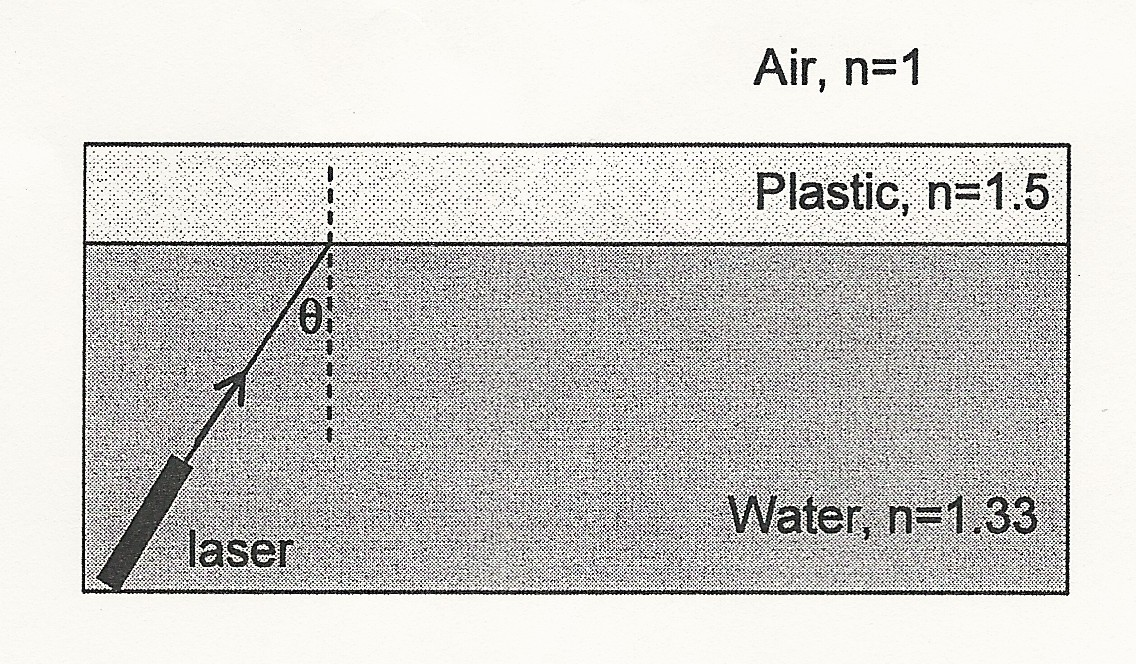
\includegraphics[scale=0.2]{Images/slab_of_water_and_plastic.jpg}
\end{center}

$\Rightarrow 48.75^\circ$

\subsection{Refraction \#2}
Light is incident on a transparent surface at an angle of $32^\circ$ with respect to the horizontal.  The refracted and reflected beams are perpendicular with each other.  What is the index of refraction of the material?  You may assume it is sitting in air (n = 1.00). \\* \\*
$\Rightarrow$ n = 1.60

\subsection{Refraction \#3}
A beam of light is incident on a material as shown below.  In the diagram, $n_1 = 1.00$, $n_2 = 1.47$, and $\theta_1 = 28.9^\circ$.  Calculate $\theta_2$.

\begin{center}
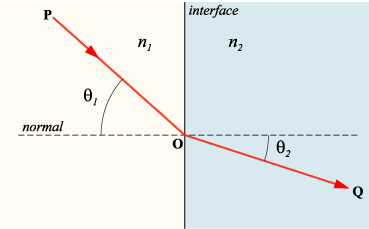
\includegraphics[scale=0.65]{Images/snells_law.png}
\end{center}

$\Rightarrow \theta_2 = 19.2^\circ$


%%%%%%%%%%%%%%%%%%%%%%%%%%%%%%%%%%%%%%%%%%%%%%%%%%%%%%%%%%%%%%%%%%%%%%%%%%%%%%%

\end{document}